\documentclass[12pt]{article}
\usepackage[left=1cm, right=1cm, top=2cm,bottom=1.5cm]{geometry} 

\usepackage[parfill]{parskip}
\usepackage[utf8]{inputenc}
\usepackage[T2A]{fontenc}
\usepackage[russian]{babel}
\usepackage{enumitem}
\usepackage[normalem]{ulem}
\usepackage{amsfonts, amsmath, amsthm, amssymb, mathtools}

\usepackage{fancyhdr}
\pagestyle{fancy}
\renewcommand{\headrulewidth}{1.5pt}
\renewcommand{\footrulewidth}{1pt}

\usepackage{graphicx}
\usepackage[figurename=Рис.]{caption}
\usepackage{subcaption}
\usepackage{float}

%%Наименование папки откуда забирать изображения
\graphicspath{ {./images/} }

%%Изменение формата для ввода доказательства
\renewcommand{\proofname}{$\square$  \nopunct}
\renewcommand\qedsymbol{$\blacksquare$}

\addto\captionsrussian{%
	\renewcommand{\proofname}{$\square$ \nopunct}%
}
%% Римские цифры
\newcommand{\RN}[1]{%
	\textup{\uppercase\expandafter{\romannumeral#1}}%
}

\theoremstyle{definition}
\newtheorem{defn}{Опр:}
\newtheorem{rem}{Rm:}
\newtheorem{prop}{Утв.}
\newtheorem{exrc}{Упр.}
\newtheorem{lemma}{Лемма}
\newtheorem{theorem}{Теорема}
\newtheorem{corollary}{Следствие}
\newenvironment{cusdefn}[1]
{\renewcommand\thedefn{#1}\defn}
{\enddefn}

\DeclareRobustCommand{\divby}{%
	\mathrel{\text{\vbox{\baselineskip.65ex\lineskiplimit0pt\hbox{.}\hbox{.}\hbox{.}}}}%
}

\newcommand{\smallerrel}[1]{\mathrel{\mathpalette\smallerrelaux{#1}}}
\newcommand{\smallerrelaux}[2]{\raisebox{.1ex}{\scalebox{.75}{$#1#2$}}}
\newcommand{\smallin}{\smallerrel{\in}}
\newcommand{\smallnotin}{\smallerrel{\notin}}


\begin{document}
	\lhead{Математический анализ - I}
	\chead{Шапошников С.В.}
	\rhead{Лекция - 6}

	
\section*{Множество вещественных чисел}


\begin{defn}
	Множество $F$ с операциями $+$ и $\cdot$ называется \uwave{полем}, если выполняются следующие условия:
	\begin{enumerate}
		\item $(F,+)$ - абелева группа:
		\begin{enumerate}
			\item $\forall a,b,c \in F, \, a + (b + c) = (a + b) + c$ (ассоциативность);
			\item $\exists \, 0\colon \, \forall a \in F, \, 0 + a = a + 0 = a$ (существование нулевого элемента);
			\item $\forall a \in F, \, \exists (-a)\colon a +(-a) = (-a) + a = 0$ (существование обратного элемента);
			\item $\forall a,b \in F, \; a + b = b + a$ (абелевость);
		\end{enumerate}
		\item $(F\setminus\{0\},\cdot)$ - абелева группа:
		\begin{enumerate}
			\item $\forall a,b,c \in F, \, a \cdot (b \cdot c) = (a \cdot b) \cdot c$ (ассоциативность);
			\item $\exists \, 1 \neq 0\colon \, \forall a \in F, \, 1 \cdot a = a \cdot 0 = a$ (существование нулевого элемента);
			\item $\forall a \neq 0 \in F, \, \exists a^{-1}\colon a \cdot a^{-1} = a^{-1} \cdot a = 1$ (существование обратного элемента);
			\item $\forall a,b \in F, \, a \cdot b = b \cdot a$ (абелевость);
		\end{enumerate}
		\item $a\cdot(b + c) = a \cdot b + a \cdot c$ (дистрибутивность);
	\end{enumerate}
\end{defn}

\textbf{Примеры полей:} 
\begin{enumerate}[label={(\arabic*)}]
	\item $\mathbb{Q}$ - множество рациональных чисел (см. книгу Ландау для проверки свойств);
	\item $\mathbb{Z}_p$, $p$ - простое;
\end{enumerate}

Рассмотрим $\mathbb{Z}_p \colon \; m \sim n \Longleftrightarrow m - n \divby p$ (одинаковые остатки при делении на $p$).\\
Классы эквивалентности: $0, 1, 2, \dotsc , p-1$ - остатки при делении на $p$. Можно проверить, что $\mathbb{Z}_p$ ($p$ - простое) - является полем.\\
В поле $\mathbb{Z}_p$ есть свойство $\underbrace{1 + 1 + \dotsc + 1}_\text{p} = 0$ в таком случае говорят, что \uwave{задано поле характеристики $p$}. Если ноль никогда не получают, то говорят, что поле - характеристики $0$.

$\mathbb{Z}_p \Rightarrow \underbrace{1 + 1 + \dotsc + 1}_\text{p} = 0$ - поле характеристики $p$.\\
$\mathbb{Q} \Rightarrow 1, \, 1 + 1, \, 1 + 1 + 1, \, \dotsc$ - не будет $0$, то есть это поле характеристики $0$ (надо $0$ раз сложить $1$).
\begin{defn}
	Поле $F$ называется \uwave{упорядоченным}, если на $F$ задан линейный порядок (любые два элемента можно сравнивать), такой, что:
	\begin{enumerate}[label={\arabic*)}]
		\item $\forall a,b,c \in F, \, a \leq b \Leftrightarrow a + c \leq b + c$;
		\item $\forall a,b,c \in F, \, a \leq b \wedge c \geq 0 \Rightarrow ac \leq bc$;
	\end{enumerate}
\end{defn}

\textbf{Пример упорядоченного поля:} $\mathbb{Q}$ - множество рациональных чисел.
\begin{prop}
 $1 > 0$
\end{prop}
	\begin{proof}
		Предположим противное $1<0 \Rightarrow$ вычитаем $1$ справа и слева $\Rightarrow 0 < -1 \Rightarrow$ умножим на ($-1$) $\Rightarrow$ по второму свойству $0<1$ - противоречие.
	\end{proof}

Тогда по свойству ($1$) получим, что $1 + 1 > 1 > 0$ и так далее. Поэтому упорядоченное поле всегда имеет характеристику поля $0$.

\begin{rem}
	Элементы упорядоченного поля: $1, 1 + 1, \dotsc ,\,\underbrace{1 + 1 + \dotsc + 1}_\text{n}, \dotsc	$ отождествляются с множеством натуральных чисел и обозначаются $\mathbb{N}$. (см. В.А. Зорич, 1-ый том для формального отождествления - индуктивные множества).		
\end{rem}
\begin{rem}
	Элементы вида $\dfrac{m}{n} = m \cdot n^{-1}$, где $m \in \mathbb{Z} = \mathbb{N} \cup \{-n \; | \; n \in \mathbb{N}\}$ и $n \in \mathbb{N}$ называем \uwave{дробями}, а их множество - \uwave{множеством рациональных чисел} $\mathbb{Q}$.
\end{rem}

\begin{defn}
	Множество $\mathbb{R}$ называется \uwave{множеством действительных} или \uwave{множеством вещественных чисел}, если $\mathbb{R}$ - упорядоченное поле, на котором выполняется \textbf{аксиома полноты}:
	
	Если $A \subset \mathbb{R}, \, A \neq \varnothing$, $B \subset \mathbb{R}, \, B \neq \varnothing$ и ``$A \leq B$'' (то есть $a \leq b, \, \forall a \in A,\, b \in B$), то $\exists c \in \mathbb{R}$, которое разделяет $A$ и $B$, то есть $a \leq c \leq b, \, \forall a \in A,\, b \in B$.
\end{defn}

\begin{figure}[H]
	\centering
	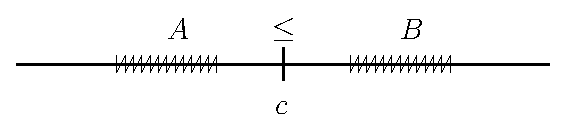
\includegraphics[width=0.40\textwidth]{6_1.eps}
	\caption{Аксиома полноты}
	\label{fig:6_1}
\end{figure}
Смысл аксиомы полноты - дырок нет. Где есть дыры? Зачем аксиома полноты?
\begin{prop}
	В $\mathbb{Q}$ существуют дыры.
\end{prop}

Например, между $A = \{\,x : x > 0 \wedge x^2 < 2\,\}$ и $B = \{\,x : x > 0 \wedge x^2 > 2\,\}$ нет элементов из $\mathbb{Q}$.

\begin{proof}
Проверим, что $A \leq B$: $x^2 < 2, \, y^2 > 2 \Rightarrow y^2 > x^2 \Rightarrow y^2 - x^2 > 0, \, (y-x)\underbrace{(y+x)}_\text{> 0} > 0 \Rightarrow y-x>0 \Rightarrow y >x$.

Пусть $\exists c \colon \, A \leq c \leq B \Rightarrow$ рассмотрим $3$ варианта: ($1$) $c^2 > 2$, ($2$) $c^2 < 2$, ($3$) $c^2 = 2$. Покажем, что ни один из них - невозможен:\\
($3$) $c^2 = 2$, представим $c$ в виде $c = \dfrac{p}{q}$ - не сократима (так как рассматриваем множество рациональных чисел) т.е. НОД($p,q$) = 1 $\Rightarrow p^2 = 2q^2 \Rightarrow p = 2k$, так как в квадрате только четные числа дают четные. Тогда $4k^2 = 2q^2 \Leftrightarrow 2k^2 = q^2 \Rightarrow q = 2m$, получили, что $p$ и $q$ $\divby 2 \Rightarrow$ противоречие.

($2$) $c^2 < 2$. Найдем $\varepsilon > 0 \colon \; (c + \varepsilon)^2 < 2$
\begin{figure}[H]
	\centering
	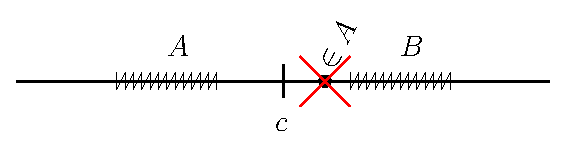
\includegraphics[width=0.4\textwidth]{6_2.eps}
	\caption{Невозможность сценария ($2$)}
	\label{fig:6_2}
\end{figure}
$c^2 + 2c\varepsilon + \varepsilon^2 < 2 \Rightarrow 2c\varepsilon + \varepsilon^2 < \underbrace{2-c^2}_\text{> 0}$ тогда $\varepsilon(2c + \varepsilon) < 2-c^2$.
Пусть $0 < \varepsilon < 1$ - поскольку мы можем выбрать $\varepsilon$. Поэтому достаточно найти такое $\varepsilon$, что будет выполнено $\varepsilon(2c + \varepsilon) < \varepsilon(2c + 1) < 2-c^2$. Возьмем $\varepsilon = \dfrac{2-c^2}{(2c+1)2017} \Rightarrow$  $c + \varepsilon \in A$ и $ c+ \varepsilon > c$, а это противоречие с тем, что $A \leq c$.\\
(1) - упражнение - доказать, что и это невозможно.\\
$c^2 > 2$. Найдем $\varepsilon > 0 \colon \; (c - \varepsilon)^2 > 2 \Rightarrow c^2 - 2c\varepsilon + \varepsilon^2 > 2 \Rightarrow  2c\varepsilon - \varepsilon^2  < \underbrace{c^2-2}_\text{> 0}$ тогда $\varepsilon(2c - \varepsilon ) < c^2 - 2$.
Пусть $0 < \varepsilon < 1$ - поскольку мы можем выбрать $\varepsilon$. Поэтому достаточно найти такое $\varepsilon$, что будет выполнено $\varepsilon(2c - \varepsilon) < 2c\varepsilon < c^2 - 2$. Возьмем $\varepsilon = \dfrac{c^2 - 2}{(2c)2017} \Rightarrow$  $c - \varepsilon \in B$ и $ c - \varepsilon < c$, а это противоречие с тем, что $c \leq B$.\\
Следовательно нет рационального числа, которое бы разделяло эти два множества.
\end{proof}
\begin{prop}
	В $\mathbb{R}$ существует $x>0 \colon \; x^2 = 2$, это $\sqrt{2}$.
\end{prop}
\begin{proof}
	Доказали в предыдущем утв. по аксиоме полноты есть $c$ которое разделяет $A$ и $B$. Доказали, что не может быть $c^2 > 2$ и $c^2 < 2$, а значит оно равно 2 ($c^2 = 2 \Rightarrow c = \sqrt{2}$).
\end{proof}

\section*{Бесконечные десятичные дроби}
\begin{defn}
	\uwave{Бесконечные десятичные дроби} - это набор последовательностей вида $a_0{,}a_1a_2\dotsc a_n$, где $a_0 \in \mathbb{Z}$, $a_k \in \{0, 1, \dotsc ,9\}$, $k \geq 1$.
\end{defn}

Последовательности с $9999\dotsc$ начиная с некоторого номера - запрещены. Почему запрещаем?\\
\textbf{Пример}: $10 \cdot 0{,}999\dotsc = 9{,}999\dotsc = 9 + 0{,}999\dotsc \Leftrightarrow 10x = 9 + x$. Тогда получим, что $0{,}999\dotsc = 1$.

\subsection*{Отношения порядка}
$a_0{,}a_1a_2\dotsc \leq b_0{,}b_1b_2\dotsc$, когда $a_0, b_0 \geq 0$ (остальные случаи - как в школе). 
Либо $a_0 < b_0$, либо $a_0 = b_0$ и $a_1 < b_1$, либо $a_0 = b_0, \, a_1 = b_1$ и $a_2 < b_2$, либо $\dotsc$ - \uwave{лексикографический порядок}.

Сложение, умножение вводятся достаточно сложно - об этом можно прочитать в книжках Садовничего (Садовничий, Ильин).

\begin{theorem}
Справедливы следующие утверждения:
\begin{enumerate}
	\item На множестве бесконечных десятичных дробей выполняется аксиома полноты;
	\item Множество бесконечных десятичных дробей является моделью множества $\mathbb{R}$ (без доказательства);
\end{enumerate}
\end{theorem}
\begin{proof}
	Проведем доказательство в случае когда $A$ и $B$ состоят из неотрицательных чисел.\\
	По условию: $A \neq \varnothing$, $B \neq \varnothing$ и $A \leq B$. Строим разделитель $c = c_0{,}c_1c_2\dotsc$, где $c_0$ - минимальное $b_0$, которое встречается в $B$ (т.к. неотрицательные числа). 
	
	Теперь смотрим только на дроби в $B$, которые начинаются с $c_0{,}\dotsc$. \\
	$c_1$ - это минимальное $b_1$, которое встречается в $B$ в дробях вида $c_0{,}b_1\dotsc$.\\
	$c_2$ - это минимальное $b_2$, которое встречается в $B$ в дробях вида $c_0{,}c_1b_2\dotsc$.
	
	Докажем, что построенная дробь $c = c_0{,}c_1c_2c_3\dotsc$ разделяет $A$ и $B$. Ясно, что $c \leq b$, $\forall b \in B$. Возьмем $b_0{,}b_1b_2\dotsc$ и сравним с $c$. $c_0 \leq b_0$, $c_1 \leq b_1$, $c_2 \leq b_2$ и так далее - по построению. Поэтому $c \leq b$, $\forall b \in B$.
	
	Возьмем $a_0{,}a_1\dotsc a_n\dotsc \in A$. Может ли случиться $a_0 > c_0$? - нет, так как тогда $a_0{,}a_1 \dotsc  >$ дроби из $B$, начинающеся с $c_0{,}\dotsc$. Пусть $a_0 = c_0$, может ли $a_1 > c_1$? - нет, так как тогда $a_0{,}a_1a_2 >$ дроби из $B$, начинающеся с $c_0{,}c_1\dotsc$ и так далее.
	
	Осталось проверить, что $c_0{,}c_1c_2\dotsc$ - допустимая запись, то есть нет $\dotsc999\dotsc$ в конце. Пусть есть, но каждый раз брали наименьшую часть $\Rightarrow c_0{,}c_1c_2\dotsc c_n9999\dotsc$, но такой записи в $B$ - нет, иначе в $B$ в дроби начиная с некоторого момента будут идти только $9$.
\end{proof}

Аксиома полноты - тяжела для проверки на практике. Поэтому её обычно переформулируют.

\begin{defn}
	Если $c \geq a, \,\forall a \in A$, то $c$ - называется \uwave{верхней гранью $A$}.
\end{defn}
\begin{defn}
	Если у $A$ есть хотя бы одна верхняя грань, то $A$ называется \uwave{ограниченным сверху множеством}.
\end{defn}
\begin{defn}
	Наименьшая из верхних граней множества $A$ называется \uwave{точной верхней гранью} множества $A$ и обозначается $\sup{A}$.
\end{defn}

\begin{defn}
	Если $c \leq a, \,\forall a \in A$, то $c$ - называется \uwave{нижней гранью $A$}.
\end{defn}
\begin{defn}
	Если у $A$ есть хотя бы одна нижняя грань, то $A$ называется \uwave{ограниченным снизу множеством}.
\end{defn}
\begin{defn}
	Наименьшая из нижних граней множества $A$ называется \uwave{точной нижней гранью} множества $A$ и обозначается $\inf{A}$.
\end{defn}

Иллюстрация определений:
\begin{figure}[H]
	\centering
	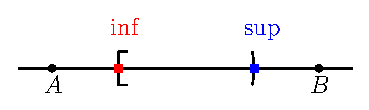
\includegraphics[width=0.3\textwidth]{6_3.eps}
	\caption{Грани множеств: $A$ - нижняя грань, $B$ - верхняя грань}
	\label{fig:6_4}
\end{figure}

\begin{theorem}\textbf{Принцип полноты Вейрштрасса}:\\
	 Если $A \neq \varnothing$ и ограничено сверxу, то $\exists \sup A$. Если $A \neq \varnothing$ и ограничено снизу, то $\exists \inf A$.
\end{theorem}
\begin{proof}
Пусть $B = \{\,\text{верхние грани}\,\}$, $A \neq \varnothing$ - по условию, $B \neq \varnothing$ - так как $A$ ограничено сверху $\Rightarrow A \leq B$. По аксиоме полноты существует разделитель $c \colon A \leq c \leq B$. $c \geq A \Rightarrow$ это верхняя грань. $c \leq B \Rightarrow$ это наименьшая верхняя грань $\Rightarrow c = \sup A$.

Пусть $B = \{\,\text{нижние грани}\,\}$, $A \neq \varnothing$ - по условию, $B \neq \varnothing$ - так как $A$ ограничено снизу $\Rightarrow B \leq A$. По аксиоме полноты существует разделитель $c \colon B \leq c \leq A$. $c \leq A \Rightarrow$ это нижняя грань. $B \leq c \Rightarrow$ это наибольшая нижняя грань $\Rightarrow c = \inf A$.
\end{proof}

\end{document}